\documentclass[a4]{article}
\usepackage{xstring}
\usepackage{graphicx}
\usepackage{tikz}
\usetikzlibrary{calc}
\usepackage{helvet}
\usepackage{geometry}
\geometry{verbose,tmargin=30pt,bmargin=90pt,lmargin=90pt,
rmargin=90pt}

%    Column B contains numbers 1 - 15
%    Column I contains numbers 16 - 30
%    Column N contains numbers 31 - 45
%    Column G contains numbers 46 - 60
%    Column O contains numbers 61 - 75

\def\NumOfColumns{5}%
\def\Sequence{1, 2, 3, 4, 5}%

\renewcommand*{\familydefault}{\sfdefault}


\newcommand{\Size}{3cm}
\tikzset{Square/.style={
    inner sep=0pt,
    text width=\Size*0.8, 
    minimum size=\Size,
    draw=black,
    fill=white,
    align=center,
    }
    %node/.style={inner sep=0,outer sep=1}
}


\begin{document}
\pagenumbering{gobble}



\begin{figure}[h]
    \centering
    
\includegraphics[width=5cm]{./mhdlogo.jpg}
\end{figure}


\section*{Bingo Instructions and Rules}
\begin{itemize}
\setlength{\itemsep}{0pt}%
\item Can't mark off a square until hack has been presented.
\item Only one square per hack, even if it qualifies for multiple squares.
\item Win by crossing off 5 in a row (diagonals accepted).
\item Declare bingo by tweeting or messaging in IRC \#mhdbingo.
\item Keep playing until the prizes run out.
\end{itemize}

\vspace{0.25cm}

\begin{center}
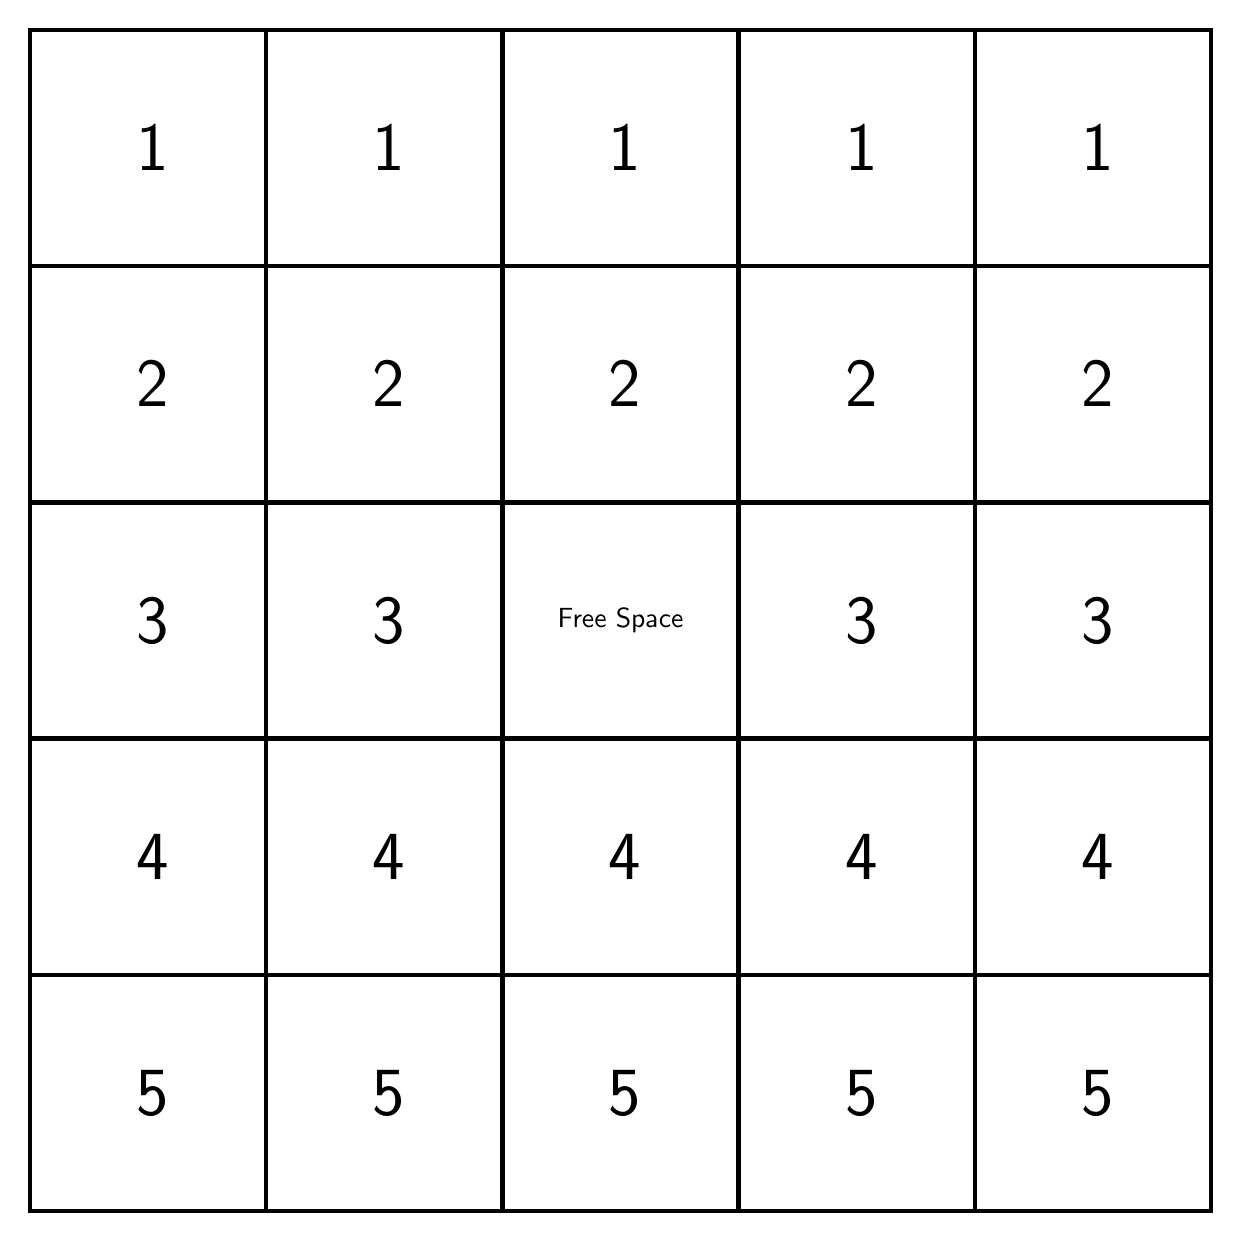
\begin{tikzpicture}[draw=black, ultra thick, x=\Size,y=\Size]
    \foreach \row in \Sequence{%
        \foreach \col in \Sequence {%
            \def\NodeText{ \row }
            \pgfmathsetmacro{\ColRowProduce}{\col*\row}
            \IfEq{\ColRowProduce}{9}{% If is center square
                \node [Square] at ($(\col,-\row)-(0.5,0.5)$) { Free Space};
            }
            {
                \node [Square] at ($(\col,-\row)-(0.5,0.5)$) { \Huge \NodeText};
            }
        }
    }
\end{tikzpicture}
\end{center}

\vspace{0.25cm}
\noindent
Thanks to @plamere, @alsothings, @sydlawrence, @xhochy, @karltryggvason, @miguelpellitero for their financial support towards prizes and printing!
\vspace{0.25cm}

\noindent
See https://www.hackerleague.org/hackathons/music-hack-day-london-2013/hacks/mhd-bingo for more info.
\end{document}